%Version 3 October 2023
% See section 11 of the User Manual for version history
%
%%%%%%%%%%%%%%%%%%%%%%%%%%%%%%%%%%%%%%%%%%%%%%%%%%%%%%%%%%%%%%%%%%%%%%
%%                                                                 %%
%% Please do not use \input{...} to include other tex files.       %%
%% Submit your LaTeX manuscript as one .tex document.              %%
%%                                                                 %%
%% All additional figures and files should be attached             %%
%% separately and not embedded in the \TeX\ document itself.       %%
%%                                                                 %%
%%%%%%%%%%%%%%%%%%%%%%%%%%%%%%%%%%%%%%%%%%%%%%%%%%%%%%%%%%%%%%%%%%%%%

%%\documentclass[referee,sn-basic]{sn-jnl}% referee option is meant for double line spacing

%%=======================================================%%
%% to print line numbers in the margin use lineno option %%
%%=======================================================%%

%%\documentclass[lineno,sn-basic]{sn-jnl}% Basic Springer Nature Reference Style/Chemistry Reference Style

%%======================================================%%
%% to compile with pdflatex/xelatex use pdflatex option %%
%%======================================================%%

%%\documentclass[pdflatex,sn-basic]{sn-jnl}% Basic Springer Nature Reference Style/Chemistry Reference Style


%%Note: the following reference styles support Namedate and Numbered referencing. By default the style follows the most common style. To switch between the options you can add or remove �Numbered� in the optional parenthesis. 
%%The option is available for: sn-basic.bst, sn-vancouver.bst, sn-chicago.bst%  
 
%%\documentclass[sn-nature]{sn-jnl}% Style for submissions to Nature Portfolio journals
%%\documentclass[sn-basic]{sn-jnl}% Basic Springer Nature Reference Style/Chemistry Reference Style
%\documentclass[sn-mathphys-num]{sn-jnl}% Math and Physical Sciences Numbered Reference Style 
\documentclass[sn-mathphys]{sn-jnl}% Math and Physical Sciences Author Year Reference Style

%\documentclass{sn-jnl}



%%\documentclass[sn-aps]{sn-jnl}% American Physical Society (APS) Reference Style
%%\documentclass[sn-vancouver,Numbered]{sn-jnl}% Vancouver Reference Style
%%\documentclass[sn-apa]{sn-jnl}% APA Reference Style 
%%\documentclass[sn-chicago]{sn-jnl}% Chicago-based Humanities Reference Style

%%%% Standard Packages
%%<additional latex packages if required can be included here>

\usepackage{graphicx}%
\usepackage{multirow}%
\usepackage{amsmath,amssymb,amsfonts}%
\usepackage{amsthm}%
\usepackage{mathrsfs}%
\usepackage[title]{appendix}%
\usepackage{xcolor}%
\usepackage{textcomp}%
\usepackage{manyfoot}%
\usepackage{booktabs}%
\usepackage{algorithm}%
\usepackage{algorithmicx}%
\usepackage{algpseudocode}%
\usepackage{listings}%

\usepackage{amssymb}
\usepackage{amsthm}
\usepackage{amsmath}
\usepackage{subfigure}
\usepackage{hyperref}
\hypersetup{pdfauthor=author}
%\usepackage{algorithm}
%\usepackage{algpseudocode}
\usepackage{booktabs}
\usepackage{caption}
\usepackage{setspace}
%\usepackage[dvipsnames]{xcolor}
%\usepackage{mathtools}

%\doublespacing

%\algdef{SE}[DOWHILE]{Do}{doWhile}{\algorithmicdo}[1]{\algorithmicwhile\ #1}%
%\algtext*{EndWhile}
%\algtext*{EndIf}
%\algtext*{EndFor}
%\algtext*{EndFunction}

% Following three lines are needed for this document.
% If you are not loading colors or url, then these are
% not required.
\usepackage{url}

\newtheorem{lemma}{Lemma}
%\newtheorem{theorem}{Theorem}
%\newtheorem{definition}{Definition}
\newtheorem{corollary}{Corollary}
%\newtheorem{proposition}{Proposition}

%\algrenewcommand\algorithmicindent{0.8em}%

%\SetKwRepeat{Do}{do}{while}fi

%\DeclareCaptionFormat{algor}{%
%  \hrulefill\par\offinterlineskip\vskip1pt%
%    \textbf{#1#2}#3\offinterlineskip\hrulefill}
%\DeclareCaptionStyle{algori}{singlelinecheck=off,format=algor,labelsep=space}

\usepackage{amsmath}
\DeclareMathOperator*{\argmax}{arg\,max}
\DeclareMathOperator*{\argmin}{arg\,min}

%\usepackage[noend]{algorithm2e}



%%%%

%%%%%=============================================================================%%%%
%%%%  Remarks: This template is provided to aid authors with the preparation
%%%%  of original research articles intended for submission to journals published 
%%%%  by Springer Nature. The guidance has been prepared in partnership with 
%%%%  production teams to conform to Springer Nature technical requirements. 
%%%%  Editorial and presentation requirements differ among journal portfolios and 
%%%%  research disciplines. You may find sections in this template are irrelevant 
%%%%  to your work and are empowered to omit any such section if allowed by the 
%%%%  journal you intend to submit to. The submission guidelines and policies 
%%%%  of the journal take precedence. A detailed User Manual is available in the 
%%%%  template package for technical guidance.
%%%%%=============================================================================%%%%

%% as per the requirement new theorem styles can be included as shown below
\theoremstyle{thmstyleone}%
\newtheorem{theorem}{Theorem}%  meant for continuous numbers
%%\newtheorem{theorem}{Theorem}[section]% meant for sectionwise numbers
%% optional argument [theorem] produces theorem numbering sequence instead of independent numbers for Proposition
\newtheorem{proposition}[theorem]{Proposition}% 
%%\newtheorem{proposition}{Proposition}% to get separate numbers for theorem and proposition etc.

\theoremstyle{thmstyletwo}%
\newtheorem{example}{Example}%
\newtheorem{remark}{Remark}%

\theoremstyle{thmstylethree}%
\newtheorem{definition}{Definition}%

\raggedbottom
%%\unnumbered% uncomment this for unnumbered level heads

\begin{document}

\title[The Conditioning Bias in Binary Decision Trees and Random Forests and Its Elimination]{The Conditioning Bias in Binary Decision Trees and Random Forests and Its Elimination}

%%=============================================================%%
%% GivenName	-> \fnm{Joergen W.}
%% Particle	-> \spfx{van der} -> surname prefix
%% FamilyName	-> \sur{Ploeg}
%% Suffix	-> \sfx{IV}
%% \author*[1,2]{\fnm{Joergen W.} \spfx{van der} \sur{Ploeg} 
%%  \sfx{IV}}\email{iauthor@gmail.com}
%%=============================================================%%

\author[1]{\fnm{G\'abor} \sur{Tim\'ar}}\email{gtimar@ua.pt}

\author*[2]{\fnm{Gy\"orgy} \sur{Kov\'acs}}\email{gyuriofkovacs@gmail.com}
%\equalcont{These authors contributed equally to this work.}

%\author[1,2]{\fnm{Third} \sur{Author}}\email{iiiauthor@gmail.com}
%\equalcont{These authors contributed equally to this work.}

\affil[1]{\orgdiv{Departamento de F\'isica}, \orgname{Universidade de Aveiro \& I3N}, \orgaddress{\street{Campus Universit\'ario de Santiago}, \city{Aveiro}, \postcode{3810-193}, \country{Portugal}}}

\affil*[2]{\orgname{Analytical Minds Ltd.}, \orgaddress{\street{\'Arp\'ad street 5.}, \city{Beregsur\'any}, \postcode{4933}, \country{Hungary}}}

%\affil[3]{\orgdiv{Department}, \orgname{Organization}, \orgaddress{\street{Street}, \city{City}, \postcode{610101}, \state{State}, \country{Country}}}

%%==================================%%
%% Sample for unstructured abstract %%
%%==================================%%

\abstract{Decision tree and random forest classification and regression are among the most widely used techniques in machine learning. Binary decision tree implementations commonly employ conditioning in the form of 'feature $\leq$ (or $<$) threshold', with the threshold being the mid-point between two observed feature values. In this paper, we investigate the bias introduced by the conditioning operator -- an intrinsic property of implementations -- when certain features have values from a small and equidistant domain. We propose techniques to eliminate this bias, necessitating an additional prediction step with decision trees but incurring no additional cost for random forests. Using 20 classification and 20 regression datasets, we demonstrate that this bias can lead to statistically significant differences in terms of AUC and $r^2$ scores. The proposed techniques successfully mitigate the bias; compared to the worst-case scenario, statistically significant improvements of up to 0.1-0.2 percentage points in AUC and $r^2$ scores were achieved, with an improvement of 1.5 percentage points in the $r^2$ score measured in the most sensitive case of random forest regression. The implementation of this study is available on GitHub at the following repository: \url{https://github.com/gykovacs/conditioning_bias}.}

%%================================%%
%% Sample for structured abstract %%
%%================================%%

% \abstract{\textbf{Purpose:} The abstract serves both as a general introduction to the topic and as a brief, non-technical summary of the main results and their implications. The abstract must not include subheadings (unless expressly permitted in the journal's Instructions to Authors), equations or citations. As a guide the abstract should not exceed 200 words. Most journals do not set a hard limit however authors are advised to check the author instructions for the journal they are submitting to.
% 
% \textbf{Methods:} The abstract serves both as a general introduction to the topic and as a brief, non-technical summary of the main results and their implications. The abstract must not include subheadings (unless expressly permitted in the journal's Instructions to Authors), equations or citations. As a guide the abstract should not exceed 200 words. Most journals do not set a hard limit however authors are advised to check the author instructions for the journal they are submitting to.
% 
% \textbf{Results:} The abstract serves both as a general introduction to the topic and as a brief, non-technical summary of the main results and their implications. The abstract must not include subheadings (unless expressly permitted in the journal's Instructions to Authors), equations or citations. As a guide the abstract should not exceed 200 words. Most journals do not set a hard limit however authors are advised to check the author instructions for the journal they are submitting to.
% 
% \textbf{Conclusion:} The abstract serves both as a general introduction to the topic and as a brief, non-technical summary of the main results and their implications. The abstract must not include subheadings (unless expressly permitted in the journal's Instructions to Authors), equations or citations. As a guide the abstract should not exceed 200 words. Most journals do not set a hard limit however authors are advised to check the author instructions for the journal they are submitting to.}

\keywords{decesion tree, random forest, bias, conditioning}

%%\pacs[JEL Classification]{D8, H51}

\pacs[MSC Classification]{62H30, 68T01, 68T05, 62D99, 62G99}

\maketitle

\section{Introduction}

Decision trees for supervised machine learning problems have been proposed more than 40 years ago \citep{chaid-earlier, id3}, and they remain preferred techniques when the interpretability of predictive models is a requirement, especially in fields such as medical \citep{dt-medicine-000, dt-medicine-001, dt-medicine-002} and financial \citep{dt-business-000, dt-business-002} decision-making. Derivative techniques, such as various types of tree ensembles (random forests \citep{rf0}, boosting \citep{xgboost, lightgbm}), are among the best-performing general-purpose classifiers and regressors, consistently outperforming other techniques in various data science problems and competitions \citep{higgs, load-forecasting}.

Decision trees are directed, acyclic graphs in which internal nodes represent tests related to the features of a problem. The branches correspond to the outcomes of these tests, and the leaf nodes contain estimates characterizing the partition of the feature space represented by the conditions along the path from the root to the leaf node. Leaf nodes typically hold class labels or probabilities for classification and continuous point estimates for regression problems. During inference, the observation vector is routed to a leaf node, and the contents of the leaf node are assigned as predictions. For an illustration, refer to Figure \ref{fig:dt}.

It was shown early on that finding the optimal decision tree for a given dataset is an NP-complete problem \citep{dt-np-complete}. Although numerous global optimization techniques \citep{evolutionary-1} and bottom-up heuristics \citep{dt-butia, dt-bottom-up} have been proposed for tree induction, top-down greedy techniques remain the most popular \citep{dt-partitioning, dt-induction}.
These approaches recursively partition the feature space by imposing equality conditions on categorical attributes or thresholding conditions on numerical attributes of the feature vectors. The conditions are optimized to decrease the impurity of target labels in the resulting partitions. In classification problems, impurity is typically measured in terms of entropy or Gini-score \citep{treebook}, while in regression problems, the primary impurity measure is usually the variance \citep{treebook}. Two variations of this scheme, C4.5 and Classification and Regression Trees (CART), are considered two of the most important algorithms in data mining \citep{top10}, with implementations available in various open-source packages such as \verb|sklearn| \citep{sklearn}, \verb|tree| \citep{tree}, and WEKA \citep{weka}, as well as commercial software like Matlab \citep{matlab} and Wolfram Mathematica \citep{mathematica}. Additionally, CART trees have proven to be efficient weak learners in highly effective ensemble techniques such as random forests \citep{rf0}, eXtreme Gradient Boosting machine (xgboost) \citep{xgboost}, and Light Gradient Boosting Machine (lightgbm) \citep{lightgbm}.

\begin{figure}
  \begin{center}
    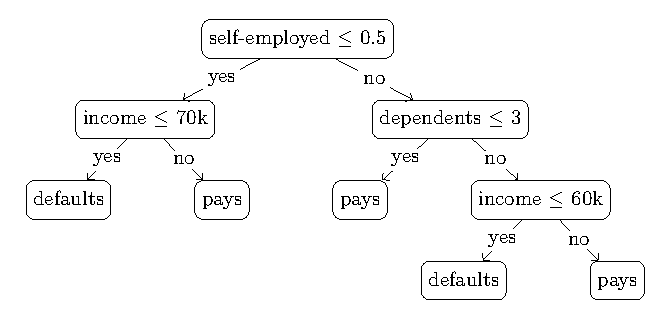
\includegraphics[width=0.67\textwidth]{forest.pdf}
  \end{center}
  \caption{A decision tree illustrating a loan approval problem, based on three features: self-employment (0 or 1), annual income, and the number of dependents. The nodes without conditions contain the prediction labels indicating whether the applicant would default or pay back the loan. For the underlying sample data, see Section \ref{sec:sample}.}
  \label{fig:dt}
\end{figure}

Although the concept of supervised decision trees is well-established, ongoing research in the field continues to introduce new ideas. Recently, impurity measures that address certain biases of conventional ones have been proposed. Examples include mutual information \citep{dt-entropy-split-mutual-information}, averaged information gain \citep{dt-average-gain}, minimum entropy of error \citep{dt-gain-minimum-entropy-of-error}, permutation statistics \citep{dt-split-others-permutation}, fuzzy rules \citep{dt-split-fuzzy}, the use of rough sets \citep{dt-split-rough-set}, and the comparison of distributions \citep{dt-chi2-0, dt-chi2-1, dt-split-ks, ds-split-ks1}. In contrast to univariate (axis-parallel) splitting functions, techniques like oblique splits \citep{dt-split-oblique, dt-split-oblique-1, oc1, hhcart} operate with multivariate splits, and the use of Support Vector Machine decision boundary for multivariate splitting has also been proposed \citep{dt-split-oblique-svm}.
Regarding regularization, various pruning techniques \citep{dt-pruning-evolutionary, dt-pruning-max-heap} have been introduced to simplify the structure of already induced decision trees. Tree learning has also been adapted for tasks beyond the classic classification and regression use cases in machine learning, such as survival rate prediction \citep{survival-forest} and density estimation \citep{density-tree}.
Finally, in line with recent trends in machine learning, research has delved into tree learning with privacy \citep{privacy}, adaptation to big data \citep{bigdata}, and the concept of deep models \citep{decision-stream}. For further details on the key concepts of decision tree learning and tree-based machine learning, we refer to \citep{treebook, survey, tutorial}.

Despite the numerous variants of decision tree learning proposed over the last decades, it is noteworthy that many applications, including those cited earlier, rely on robust implementations of binary CART decision trees (and their ensembles) \citep{sklearn, tree, caret, xgboost, lightgbm}. These tree induction techniques usually assume that all features are continuous or are embedded into a continuous representation. Thus, the partitioning of the training data and the feature space by thresholding conditions (such as the ones in Figure \ref{fig:dt}) is applicable along all axes. However, in general, the partitioning of the finite amount of training data does not imply a unique partitioning of the continuous feature space. One ambiguity arises from the fact that if there are no observations for a feature between the observed $x^l$ and $x^u$ values, any threshold $t\in]x^l, x^u[$ leads to the same partitioning of training data. This ambiguity is usually resolved in alignment with the assumption of the features being continuous: if the threshold should fall between the observed $x^l$ and $x^u$ values, the mid-point $t=(x^l + x^u)/2$ is used, thus, assigning 50\% of the unlabeled interval to both the left and right partitions. Another ambiguity arises from the choice of conditioning: the Python implementation \emph{sklearn} \citep{sklearn} uses the operator $\leq$ in the form $x \leq t$, leading to partitions open from the left and closed from the right along each axis (as in Figure \ref{fig:dt}), however, the R implementation \emph{tree} \citep{tree} uses conditions of the form $x < t$. Considering the presumption of continuous features, the choice of conditioning operator should have a marginal effect, as a feature takes the exact value of a threshold with negligible probability. However, \emph{when the domain of a feature consists of a small number of equidistant values, the thresholds determined as the mid-points of observations can be aligned with feature values, making the predictions dependent on the choice of conditioning operator and leading to a bias}.

Although it might seem to have a marginal effect, due to the popularity and numerous applications of binary decision trees and random forests, we dedicate this paper to investigating this potential bias.
The contributions of the paper to the field can be summarized as follows:
\begin{enumerate}
\item We establish and introduce the term \emph{conditioning bias}, referring to the variation of prediction outcomes depending on the choice of conditioning operator in binary decision tree implementations.
\item With statistical significance, we demonstrate the emergence of the conditioning bias in both binary decision trees and random forests when attributes taking values from small, equidistant domains are present.
\item We discuss methods for eliminating the bias, proposing various practical techniques depending on the accessibility of the internals of fitted trees for its mitigation.
\item Through extensive experiments, we demonstrate that the proposed methods reduce the bias and can lead to statistically significant improvements of up to 0.1-0.2 percentage points in AUC and $r^2$ scores, with an observed improvement of 1.5 percentage points in the most sensitive case.
\item An important finding is that the elimination of the bias in random forests incurs no additional computational costs, neither in training nor in inference time. The proposed method represents a \emph{free-lunch} improvement for applications using random forests on datasets with features susceptible to the bias.
\end{enumerate}
The proposed techniques and the completely reproducible implementation of the study are shared with the community in the GitHub repository \url{https://github.com/gykovacs/conditioning_bias}.

The paper is organized as follows: In Section \ref{sec:problem}, we formulate the problem and demonstrate its existence qualitatively. Section \ref{sec:proposed} describes the proposed solutions. The experimental setup and the results of the tests are presented and discussed in Section \ref{sec:tests}, and finally, conclusions are drawn in Section \ref{sec:summary}.

\section{Problem Formulation}
\label{sec:problem}

In this section, we provide an introduction to decision tree learning (subsections \ref{sec:problem-intro} and \ref{sec:problem-split}), and formulate the problem we address (subsection \ref{sec:problem-bias}).
Normal, boldface and calligraphic typesetting denote scalars ($d \in\mathbb{Z}$), vectors ($\mathbf{x}\in\mathbb{Z}^d$) and sets ($\mathcal{S}\subset\mathbb{Z}$), respectively. Elements of sequences and sets are indexed by superscripts, coordinates of vectors are referred by subscripts.

\subsection{Decision tree induction}
\label{sec:problem-intro}

The popular CART-type binary decision trees \citep{cart} \emph{assume all features being continuous}, and build the decision trees by recursively partitioning the training set to improve the purity of training labels within the partitions by the following steps. Let $(\mathbf{x}^i, y^i)_{i=1}^{N}, \mathbf{x}^i \in \mathbb{R}^{d}, y^i\in\mathbb{R}$ denote the feature vectors and corresponding labels. Let $\mathcal{N}\subseteq \lbrace 1, \dots, N\rbrace$ be the indices of training vectors at a particular node (initially all indices at the root node) and $I(\mathcal{N})$ be the impurity of labels $(y^i)_{i\in\mathcal{N}}$:

\begin{enumerate}
\item [S1] If the impurity of labels $I(\mathcal{N})$ is below a threshold, the node becomes a leaf node and the relevant statistics of the labels are recorded for prediction.
\item [S2] Otherwise, the best feature $f^* \in \lbrace 1, \dots, d\rbrace$ and threshold $t^* \in \mathbb{R}$ are determined  
such that partitioning the training set into left $\mathcal{L} = \lbrace j \vert  \mathbf{x}^j_{f^*} \leq t^*, j \in \mathcal{N}\rbrace$ and right $\mathcal{R} = \mathcal{N}/\mathcal{L}$ subsets minimizes the total impurity $I(\mathcal{L}) + I(\mathcal{R})$. The parameters ($f^*$, $t^*$) are recorded and left and right child nodes are added by applying step S1 to the training records indexed by $\mathcal{L}$ and $\mathcal{R}$, respectively.
\end{enumerate}
The key operation at a node is determining the optimal threshold $t$ for a feature $f$, such that conditioning the training records by $\mathbf{x}_f \leq t$, the highest impurity reduction is gained in the resulting partitions.
In practice, the feature values are sorted $\mathbf{x}^{s_1}_f \leq \dots \leq \mathbf{x}^{s_N}_f$, and the index of the rightmost value in the left partition is determined:
\begin{equation}
k^* = \argmin\limits_{\substack{k \in \lbrace 1, \dots, N - 1 \rbrace\\ \mathbf{x}^{s_{k}} \neq \mathbf{x}^{s_{k + 1}}}}I((y^{s_i})_{i=1}^{k}) + I((y^{s_i})_{i=k+1}^{N}),
\end{equation}
that is, the splitting needs to take place between $x^{s_{k^*}}_f$ and $x^{s_{k^* + 1}}_f$. 
Given that there are no observations in the interval, and in line with the assumption that the feature is continuous, most implementations choose the mid-point $t = (x^{s_{k^*}}_f + x^{s_{k^* + 1}}_f)/2$ as threshold, assigning 50\% of the splitting interval to both partitions (see Figure \ref{fig:split-cont}). We highlight that using the mid-points as thresholds, \emph{the choice of conditioning ($<$ or $\leq$) does not affect the tree induction}.
For further details on decision tree induction and  refer to \citep{treebook}.

\subsection{Inference with decision trees}
\label{sec:problem-split}

Inference for a vector $\mathbf{x}$ is conducted by starting from the root node and recursively applying the condition $\mathbf{x}_{f} \leq t$ or $\mathbf{x}_{f} < t$, with the parameters $f$ and $t$ recorded in the current node, and routing $\mathbf{x}$ to the subtree corresponding to the output of the condition. Upon encountering a leaf node, the recorded statistics (such as the class distribution for classification) are returned as the prediction for $\mathbf{x}$.
The conditioning $\mathbf{x}_f\leq t$ aligns with the Python implementation \emph{sklearn} \citep{sklearn}, while other implementations (such as the R package \emph{caret} \citep{caret}) use conditions of the form $\mathbf{x}_{f} < t$.

Unlike tree induction, \emph{inference can depend on the choice of conditioning operator}. Particularly, when a feature value coincides with a threshold, the routing of the vector depends on the conditioning. 
For example, in the tree in Figure \ref{fig:dt}, there is a split on the attribute \emph{dependents} at 3, which can occur if the training set at the root node does not contain records with 3 dependents. The routing of records with $dependents=3$ is determined by the conditioning: with $\leq$ it is routed to the left and with $<$ to the right.

Naturally, with truly continuous features, the probability of a feature value matching a threshold is negligible. However, under the following circumstances, feature values can coincide with thresholds:
\begin{enumerate}
\item \emph{A feature takes values from an equidistant domain with non-negligible probability}: the thresholds (mid-points) between observations being an even number of equidistant steps apart are also domain values.
\item \emph{Relatively deep trees are built}: a threshold can fall on a domain value only if it is missing from the training set at the respective node -- the deeper a tree gets, the smaller the training set becomes, leading to gaps in the representation of the feature domain.
\end{enumerate}
We highlight that features with a small, equidistant domains are common in practice. For instance, the \emph{age} attribute in medical datasets; \emph{rounded decimals} when features are observed to a certain number of digits; and \emph{monetary values} quoted in units of millions in financial datasets to mention a few.
We also mention that due to the regularizing effect of bootstrap aggregation, the decision trees used in random forests need less regularization by depth, consequently, random forests can be expected to be more affected by the phenomenon.

\subsection{The conditioning bias}
\label{sec:problem-bias}

It can be argued that the variation of predictions is due to using the mid-points as thresholds. However, the mid-points are reasonable choices for continuous features, any alternative would lead to asymmetries and consequent biases. Therefore, we consider the phenomenon to be \emph{an artifact of dealing with discrete features in a continuous framework}, and attribute it to the inadequacy of both conditioning operators in such cases. 

For the ease of discussion, we introduce the term \emph{conditioning bias} to refer to the variation of predictions due to the choice of conditioning.
In the rest of the paper, we address the mitigation of the conditioning bias from the theoretical and practical points of view.

\begin{figure}[t]
  \begin{center}
    \subfigure[\label{fig:split-cont-a}]{
      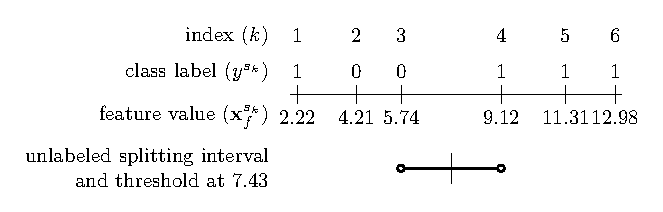
\includegraphics[width=0.67\textwidth]{continuous.pdf}}
    \subfigure[\label{fig:split-cont-b}]{
      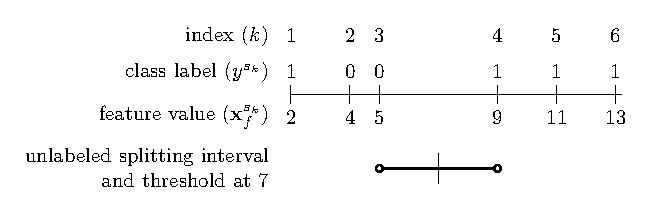
\includegraphics[width=0.67\textwidth]{discrete.pdf}
    }
  \end{center}
  \caption{Finding the optimal partitioning in a classification problem for a continuous (a) and discrete (b) feature. In both cases, $k^* = 3$ leads to the lowest Gini-impurity for the resulting partitions (0.222). 
}

  \label{fig:split-cont}
\end{figure}

\section{The Proposed Method}
\label{sec:proposed}

In this section, we introduce methods to mitigate the conditioning bias. First, in subsection \ref{sec:hyper}, we discuss the challenge of determining the impact of the conditioning operator on prediction performance and conclude that \emph{the conditioning operator should not be treated as a hyperparameter}. To eliminate the potentially detrimental effects of the conditioning bias, we propose integrating it out by making predictions with both conditioning operators and averaging the results, as detailed in subsection \ref{sec:integrate}.
In practice, most implementations typically support only one default conditioning form. Our goal is to offer practical solutions easily applicable to popular decision tree and random forest implementations, even when the internals of the trees are not readily accessible or modifiable. This is especially important in managed environments like Matlab \citep{matlab}, SAS \citep{sas}, and no-code platforms \citep{nocode}. Hence, in subsection \ref{sec:equiv}, we present various approaches to conduct predictions with the non-default conditioning operator of an implementation, without needing to adjust the inference engine.

%In this section, the proposed methods for the mitigation of the conditioning bias are presented. First, in subsection \ref{sec:hyper}, we discuss that without making further assumptions about the distribution of the data, it is not possible to decide which conditioning operator would lead to improved or deteriorated prediction performance: \emph{the conditioning operator cannot be treated as a hyperparameter}. Consequently, to eliminate the potentially detrimental effects of the conditioning bias, it needs to be integrated out by \emph{making predictions with both conditioning operators and taking the average}, that we discuss in detail in subsection \ref{sec:integrate}. 
%In practice, most implementations support only one form of conditioning by default. Our goal is to propose practical solutions that are easily applicable to popular decision tree and random forest implementations even when the internals of the trees are not or not easily accessible and mutable (for example, in managed environments, like Matlab \citep{matlab} and SAS \citep{sas} and no-code platforms \citep{nocode}). Therefore, in subsection \ref{sec:equiv}, we present various approaches to carry out predictions with the non-default conditioning operator of an implementation, without adjusting the inference engine.

\subsection{The conditioning operator as a hyperparameter}
\label{sec:hyper}

From a general perspective, the conditioning operator could be regarded as another hyperparameter of tree induction, akin to the maximum depth. In theory, one could assess both operators ($<$ and $\leq$) in a cross-validation scheme during model selection and opt for the one that yields the best performance. Additionally, it can be argued that when features susceptible to the bias are present, the conditioning operator could be optimized for each of those features, or even optimized for each affected node of the tree.

Unfortunately, proper cross-validation of the conditioning operator is challenging. Unlike real regularization parameters, such as maximum depth or leaf node size, which offer interpretable controls over smoothness, the choice of conditioning influences specific edge cases and has unpredictable effects. In a typical cross-validation scenario, potentially in an iterated manner, a certain percentage ($P\%$) of the available data is selected for training, with the remainder used for testing. If predictions with the two conditioning operators differ on some records the test set(s), it is due to feature values in the test set coinciding with thresholds at certain nodes on certain decision paths. However, once the cross-validated model selection is completed and the model is fitted to the entire dataset, the test records incorporated in the fitting remove the thresholds that coincided with feature values in the cross-validation, and other thresholds along other paths can coincide with other domain values, resulting in unpredictable effects on future, unseen data. Consequently, the cross-validated selection of the optimal conditioning leads to overfitting: \emph{the difference in the cross-validated performance of conditioning operators cannot be generalized to fitting the entire dataset}.

Nevertheless, one operator can still lead to worse performance than the other (see subsection \ref{sec:tests-quant} for a quantitative assessment of the effect size). We emphasize that in the form of the default conditioning operator, a choice is already made in popular implementations, and there is no reason to assume that there is anything other than a 50\% chance that the default operator is not detrimental to the performance in a problem when features with small, equidistant domains are present. Given the challenges of selecting the optimal conditioning operator by cross-validation, we focus on eliminating the downside risk of using an operator leading to deteriorated performance by integrating out the effect of operator choice.

\subsection{Integrating out the conditioning}
\label{sec:integrate}

A conservative yet reasonable approach to mitigate the conditioning bias is to integrate out the ambiguity. 
%As we discussed in subsection \ref{sec:hyper}, it cannot be inferred from the data which conditioning operator would beneficial or detrimental to the performance once all data is fit.
Specifically, carrying out inference with both operators and averaging their predictions effectively eliminates the dependence on the conditioning operator. This method can be expected to yield predictions at least as good as those produced by the conditioning operator with the worse performance.

With single decision trees, carrying out predictions with both conditioning operators and averaging the results is straightforward. Two aspects need further investigation: computational complexity and interpretability. In terms of computational complexity, the prediction time doubles. However, the trade-off of doubling prediction time for bias-free predictions can be favorable in numerous applications where execution time is not critical. It is worth noting that prediction with decision trees is relatively fast compared to many other machine learning techniques, such as k Nearest Neighbors (kNN), making it competitive even with the doubled prediction time.
Nevertheless, single decision trees are primarily valued for the interpretability of predictions through the decision paths they traverse during inference. When predictions obtained with the two conditioning operators follow the same decision path (i.e., thresholds do not coincide with feature values), interpretability is preserved, with each prediction having a unique decision path. However, when the decision paths differ for a particular prediction, both are equally valid. Having two differing decision paths for the same prediction clearly increases the complexity of interpretation. However, relying on a single decision path would be as misleading as the corresponding prediction being biased when feature values coincide with thresholds.
%when both are influenced by the a-priori choice of the conditioning operator.

%, as well as signaling that the prediction of these records interferes with the assumption of continuous features.

%, which would stay hidden . Relying on one conditioning operator would hide that these predictions are influenced by the choice of conditioning in the implementation.

In the case of random forests, one can follow the same approach and evaluate each tree of the ensemble with both operators and average the results, which would double the prediction time. However, given the typically large number of estimators, evaluating half of the trees with the default operator and the other half with the non-default conditioning should be a reasonably accurate approximation, which does not increase the prediction time, at all. Consequently, in the case of random forests, the elimination of the bias is a \emph{free lunch} improvement of the predictions. 

%Moreover, even if the tree induction implementation does not provide easy access to the internals, one can train one forest of $N_e/2$ trees on the original dataset and another forest of $N_e/2$ trees on the opposites (additive inverses) of feature vectors and use the average of the predictions for inference. 
%Consequently, the approach can improve the quality of predictions with any random forest implementation for no additional cost either in training or prediction time apart from multiplying feature vectors by $-1$ and averaging two predictions.

\subsection{Prediction with the non-default conditioning operator}
\label{sec:equiv}

In the methods we proposed, it is crucial to carry out predictions with both conditioning operators. However, in popular decision tree implementations, the conditioning operator is an intrinsic property that cannot be changed. Since decision tree induction is not affected by the conditioning operator but needs to be efficient and usually involves various advanced operations like pruning \citep{sklearn}, creating custom implementations where the conditioning operator is a parameter is impractical, especially in graphical and low/no-code machine learning environments \citep{nocode}.
To facilitate applications in any environment, in this subsection, we discuss various alternative ways to obtain predictions with the non-default operator of an implementation.

Let $\mathcal{T} = (\mathbf{x}_i, y_i)_{i=1}^N$ denote a training set, and $T_{\mathcal{T}}$ be a decision tree fitted to $\mathcal{T}$. Without loss of generality, we can suppose that the available tree induction and prediction implementation intrinsically uses the conditioning operator $\leq$. 
Let the prediction for $\mathbf{x}$ be denoted by $T_{\mathcal{T}}(\mathbf{x}, \leq)$. Our interest lies in inference with the same tree but using the non-default operator denoted as $T_{\mathcal{T}}(\mathbf{x}, <)$. As a practical example, we want to carry out inference with the tree in Figure \ref{fig:dt2-a}, given the possibility of inference with the tree in Figure \ref{fig:dt}.

The proposed workarounds to obtain $T_{\mathcal{T}}(\mathbf{x}, <)$ are based on the identity that the conditioning $\mathbf{x}_f < t$ is equivalent to $-\mathbf{x}_f \leq -t$ in the sense that if a vector $\mathbf{x}$ is routed to the left by $\mathbf{x}_f < t$, then $-\mathbf{x}$ is routed to the right by $-\mathbf{x}_f \leq -t$. Based on this identity, we introduce the operation of \emph{tree mirroring}, denoted by $\mathcal{M}[T_{\mathcal{T}}]$: interchanging the left and right subtrees and replacing the threshold $t$ with $-t$ in each node. 
The benefit of tree mirroring is that predicting $-\mathbf{x}$ with the mirrored tree leads to the same prediction along the same (but mirrored) decision path as predicting $\mathbf{x}$ by replacing the conditioning operator in the original tree. Formally, $T_{\mathcal{T}}(\mathbf{x}, <) = \mathcal{M}[T_{\mathcal{T}}](-\mathbf{x}, \leq)$.
For illustration, in Figure \ref{fig:dt2-b} we have plotted the mirrored version of the tree depicted in Figure \ref{fig:dt}. Considering a vector with a feature value coinciding with a threshold $\mathbf{x} = (\text{self-employment}: 0, \text{dependents}: 3, \text{income}: 50k)$, the predictions with the original tree (Figure \ref{fig:dt}) and the tree with the non-default operator (Figure \ref{fig:dt2-a}) lead to different results. However, the predictions using the operator $<$ (Figure \ref{fig:dt2-a}) and predicting $-\mathbf{x}$ with the mirrored tree (Figure \ref{fig:dt2-b}) are equivalent. 

Based on the equivalence of mirroring and changing the conditioning operator, and depending on the accessibility of the trained tree structure, we have identified two methods to obtain $T_{\mathcal{T}}(\mathbf{x}, <)$, without reimplementing the inference:
\begin{enumerate}
\item If \emph{the trained tree structure is accessible}, one can mirror the tree by recursively interchanging the left and right child nodes, replacing each threshold $t$ by its opposite $-t$. Then, infering $-\mathbf{x}$ with the mirrored tree leads to predictions equivalent to using the non-default conditioning operator for predicting $\mathbf{x}$ with the original tree. For example, the Python \emph{sklearn} \citep{sklearn} tree structure is easily accessible and mutable, and the mirroring operation is applicable. The benefit of mirroring is that it can be done by recursively traversing the existing tree once, which is computationally less demanding than a typical training.
\item If \emph{the trained tree structure is not or not easily accessible}, the mirrored tree can be induced directly from the training set $\mathcal{T}' = (-\mathbf{x}_i, y_i)_{i=1}^N$. We note that depending on the implementation, in the case of multiple, equally good partitionings at a certain node, the ties might be resolved randomly, leading to differences in the tree structure when the tree is fit to $\mathcal{T}'$. Apart from the differences due to tie resolution, again, infering $-\mathbf{x}$ with the tree fit to $\mathcal{T}'$ leads to predictions equivalent to using the non-default conditioning operator for predicting $\mathbf{x}$ with the tree fit to $\mathcal{T}$.
Although this approach requires an additional training with $\mathcal{T}'$, its main benefit is that it is applicable even in low/no-code machine learning environments \citep{nocode}, where the internals of trained trees are not accessible.
\end{enumerate}
With these workarounds, it becomes feasible to compare the performance of the two conditioning operators and mitigate the bias in most machine learning environments, without the need to implement custom inference engines.

%In the case of random forests, in the previous section, we argued, that half of the trees should be evaluated with both operators to keep the prediction time intact. Utilizing the mirroring property, the same effect can be achieved by simply fitting a forest half the size to the original data, and another forest of the same size to the inverses of the feature vectors, and taking the averages.


\begin{figure*}
  \begin{center}
    \subfigure[\label{fig:dt2-a}]{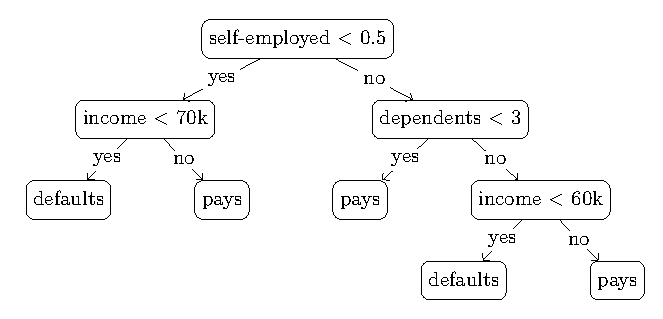
\includegraphics[width=0.67\textwidth]{forest3.pdf}}
    \subfigure[\label{fig:dt2-b}]{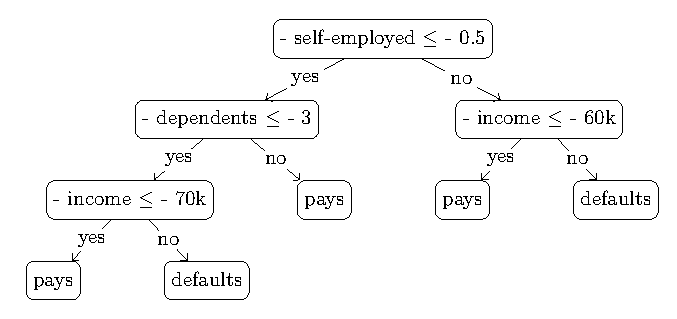
\includegraphics[width=0.67\textwidth]{forest2.pdf}}
  \end{center}
  \caption{The decision tree in Figure \ref{fig:dt} with replaced conditioning operators (a), and its mirrored variant (b). One can check that given any feature vector $\mathbf{x}$, the prediction of $\mathbf{x}$ with (a) and that of $-\mathbf{x}$ with (b) leads to the same result along the same (but mirrored) decision path.}
  \label{fig:dt2}
\end{figure*}

\section{Tests and Results}
\label{sec:tests}

In Section \ref{sec:problem}, we argued that the conditioning bias can emerge in CART-type decision trees and derivative techniques when features with small and equidistant domains are present in a dataset. Then, in Section \ref{sec:proposed}, we introduced methods to mitigate the bias. The goal of this section is twofold: (a) demonstrating the emergence of the conditioning bias and quantifying its size; (b) demonstrating that the proposed methods effectively reduce the potential performance deterioration associated with the bias. 
Given the widespread use and popularity of decision trees and random forests in machine learning, and the focus of our research on a specific characteristic of decision tree learning, we deemed comparisons to other state-of-the-art techniques unnecessary.

The section is organized as follows. We begin by presenting the datasets selected for evaluation in subsection \ref{sec:tests-datasets}. Next, we revisit the role of cross-validation in subsection \ref{sec:tests-cv} and discuss the evaluation methodology in subsections \ref{sec:tests-model} and \ref{sec:tests-testing}. The existence of the conditioning bias is demonstrated in subsection \ref{sec:tests-quant}, and finally, the proposed methods are evaluated in subsection \ref{sec:tests-proposed}.

\subsection{Datasets}
\label{sec:tests-datasets}

To facilitate the selection of datasets for testing and evaluation, we introduce a heuristic condition. We consider a feature susceptible to the conditioning bias if there exists an observed domain value $\mathbf{x}_f$ and a positive real number $r\in\mathbb{R}^+$ such that $\mathbf{x}_f-r$ and $\mathbf{x}_f+r$ are also observed. This condition ensures that at least one threshold might align with a domain value. It is worth noting that this condition is not necessary; previously unseen records can still interfere with thresholds, even if none of the features in the training data meet the condition.

We selected 20 binary classification and 20 regression datasets primarily from the UCI \citep{uci} and KEEL \citep{keel} repositories, using the criterion that each dataset should contain \emph{at least one feature susceptible to the conditioning bias}. The dataset collection preceded all experiments and was not influenced by any experimental results. As observed in Table \ref{tab:datasets}, the datasets cover approximately an order of magnitude range in both the number of training records and the number of features. Interestingly, features susceptible to the bias are more frequent in commonly used evaluation datasets than we anticipated; in many cases, all features meet the condition, despite the requirement being to have at least one such feature. To further support the claim regarding the frequency of features susceptible to the bias, it is noteworthy that the average proportion of such features within the toy datasets available in the \emph{sklearn} \citep{sklearn} package is 97\% - almost all features of all toy datasets belong to this category.

The same preprocessing steps were applied to all datasets. First, missing data imputation was performed using the most frequent value. Next, for categorical features with at most 5 categories, one-hot encoding was applied, while integer encoding was used for features with more than 5 categories. Standardization was not necessary when working with tree techniques.

\begin{table*}[t]
  \caption{A summary of the key characteristics of the datasets used for evaluation, with $N$, $N_a$ and $N_b$ representing the number of records, attributes and the number attributes susceptible to the bias, respectively. The counts of attributes were determined after the encoding of categorical attributes. $N_m$ denotes the number of minority samples in classification problems. The columns $par_{t}$ and $par_{f}$ encode the hyperparameters of the trees and forests leading to the highest AUC score ($auc_*$) or $r^2$ score ($r^2_*$). The hyperparameters indicate the minimum number of samples on the leaf nodes ($\alpha$) or the maximum depth ($\beta$), respectively. The datasets are sorted by their size $N\cdot N_a$.}
  \label{tab:datasets}
  \begin{center}
    \begin{footnotesize}
      \begin{tabular}{l@{\hspace{6pt}}r@{\hspace{6pt}}r@{\hspace{6pt}}r@{\hspace{6pt}}r@{\hspace{6pt}}l@{\hspace{6pt}}r@{\hspace{6pt}}l@{\hspace{6pt}}r}
\toprule
\multicolumn{9}{c}{Classification} \\
dataset & N & $N_a$ & $N_b$ & $N_m$ & par$_t$ & auc$_t$ & par$_f$ & auc$_f$ \\
\midrule
appendicitis \citep{keel} & 106 & 7 & 7 & 21 & $\alpha$: 16 & 0.775 & $\alpha$: 16 & 0.852 \\
haberman \citep{keel} & 306 & 3 & 3 & 81 & $\alpha$: 22 & 0.662 & $\alpha$: 13 & 0.721 \\
new-thyroid1 \citep{keel} & 215 & 5 & 5 & 35 & $\alpha$: 15 & 0.959 & $\beta$: 6 & 1.000 \\
glass0 \citep{keel} & 214 & 9 & 9 & 70 & $\alpha$: 15 & 0.837 & $\beta$: 10 & 0.929 \\
shuttle-6-vs-2-3 \citep{keel} & 230 & 9 & 9 & 10 & $\alpha$: 2 & 1.000 & $\alpha$: 1 & 1.000 \\
bupa \citep{keel} & 345 & 6 & 6 & 145 & $\alpha$: 11 & 0.695 & $\alpha$: 2 & 0.767 \\
cleveland-0-vs-4 \citep{keel} & 177 & 13 & 10 & 13 & $\alpha$: 7 & 0.898 & $\alpha$: 4 & 0.979 \\
ecoli1 \citep{keel} & 336 & 7 & 5 & 77 & $\alpha$: 31 & 0.954 & $\alpha$: 3 & 0.958 \\
poker-9-vs-7 \citep{keel} & 244 & 10 & 10 & 8 & $\alpha$: 17 & 0.682 & $\beta$: 4 & 0.986 \\
monk-2 \citep{keel} & 432 & 6 & 4 & 204 & $\alpha$: 2 & 1.000 & $\alpha$: 2 & 1.000 \\
hepatitis \citep{krnn} & 155 & 19 & 6 & 32 & $\alpha$: 6 & 0.744 & $\beta$: 2 & 0.871 \\
yeast-0-3-5-9-vs-7-8 \citep{keel} & 506 & 8 & 6 & 50 & $\alpha$: 9 & 0.737 & $\alpha$: 4 & 0.810 \\
mammographic \citep{keel} & 830 & 5 & 5 & 403 & $\alpha$: 46 & 0.900 & $\beta$: 3 & 0.912 \\
saheart \citep{keel} & 462 & 9 & 8 & 160 & $\alpha$: 25 & 0.719 & $\beta$: 3 & 0.755 \\
page-blocks-1-3-vs-4 \citep{keel} & 472 & 10 & 10 & 28 & $\alpha$: 15 & 0.976 & $\beta$: 12 & 0.999 \\
pima \citep{keel} & 768 & 8 & 8 & 268 & $\alpha$: 33 & 0.805 & $\beta$: 5 & 0.836 \\
wisconsin \citep{keel} & 683 & 9 & 9 & 239 & $\alpha$: 13 & 0.983 & $\alpha$: 2 & 0.993 \\
abalone9-18 \citep{keel} & 731 & 9 & 7 & 42 & $\alpha$: 116 & 0.758 & $\alpha$: 4 & 0.850 \\
winequality-red-3-vs-5 \citep{keel} & 691 & 11 & 11 & 10 & $\alpha$: 85 & 0.815 & $\alpha$: 17 & 0.870 \\
\bottomrule
\end{tabular}
\\
      \begin{tabular}{l@{\hspace{6pt}}r@{\hspace{6pt}}r@{\hspace{6pt}}r@{\hspace{6pt}}l@{\hspace{6pt}}r@{\hspace{6pt}}l@{\hspace{6pt}}r}
\toprule
\multicolumn{8}{c}{Regression} \\
dataset & N & $N_a$ & $N_b$ & par$_t$ & r$^2_t$ & par$_f$ & r$^2_f$ \\
\midrule
diabetes \citep{keel} & 43 & 2 & 2 & $\alpha$: 6 & -0.375 & $\beta$: 2 & -0.083 \\
o-ring \citep{uci} & 23 & 6 & 4 & $\alpha$: 1 & 0.127 & $\beta$: 2 & 0.150 \\
wsn-ale \citep{uci} & 107 & 5 & 4 & $\alpha$: 5 & 0.434 & $\alpha$: 2 & 0.561 \\
daily-demand \citep{uci} & 60 & 12 & 7 & $\alpha$: 1 & 0.697 & $\beta$: 7 & 0.828 \\
slump-test \citep{krnn} & 103 & 9 & 9 & $\alpha$: 2 & 0.623 & $\beta$: 8 & 0.769 \\
servo \citep{uci} & 167 & 10 & 2 & $\alpha$: 4 & 0.686 & $\alpha$: 2 & 0.721 \\
yacht-hydrodynamics \citep{krnn} & 307 & 6 & 6 & $\alpha$: 1 & 0.993 & $\beta$: 11 & 0.995 \\
autoMPG6 \citep{keel} & 392 & 5 & 5 & $\alpha$: 10 & 0.823 & $\beta$: 12 & 0.872 \\
excitation-current \citep{uci} & 557 & 4 & 4 & $\beta$: 10 & 1.000 & $\beta$: 11 & 1.000 \\
real-estate-valuation \citep{uci} & 414 & 6 & 5 & $\alpha$: 6 & 0.658 & $\alpha$: 4 & 0.709 \\
wankara \citep{keel} & 321 & 9 & 9 & $\alpha$: 2 & 0.972 & $\beta$: 9 & 0.987 \\
plastic \citep{keel} & 1650 & 2 & 2 & $\alpha$: 9 & 0.766 & $\alpha$: 9 & 0.789 \\
laser \citep{keel} & 993 & 4 & 4 & $\alpha$: 3 & 0.922 & $\beta$: $\infty$ & 0.963 \\
qsar-aquatic-toxicity \citep{uci} & 546 & 8 & 8 & $\alpha$: 17 & 0.355 & $\beta$: 14 & 0.525 \\
baseball \citep{keel} & 337 & 16 & 12 & $\alpha$: 8 & 0.641 & $\beta$: 5 & 0.680 \\
maternal-health-risk \citep{uci} & 1013 & 6 & 6 & $\beta$: $\infty$ & 0.713 & $\beta$: $\infty$ & 0.749 \\
cpu-performance \citep{krnn} & 209 & 35 & 6 & $\beta$: 8 & 0.812 & $\beta$: 13 & 0.870 \\
airfoil \citep{krnn} & 1503 & 5 & 4 & $\beta$: 15 & 0.861 & $\beta$: $\infty$ & 0.934 \\
medical-cost \citep{mlwithr} & 1338 & 6 & 2 & $\beta$: 3 & 0.761 & $\beta$: 3 & 0.765 \\
\bottomrule
\end{tabular}

    \end{footnotesize}
  \end{center}
\end{table*}

We note that the presence of the bias depends on the representativeness of features at certain nodes, rather than on the overall size of the training set. The bias can emerge even when a dataset consists of millions of records if sufficiently deep trees are induced.

\subsection{A note on the use of cross-validation}
\label{sec:tests-cv}

%In subsection \ref{sec:hyper}, we discussed why cross-validation cannot be employed to select the conditioning operator as part of the model selection process. Nevertheless, with the right interpretation, cross-validation remains a valuable tool for the quantitative assessment of the bias and the proposed methods: we can estimate the size of the bias, and we can determine which conditioning operator works better given that 80\% of the data is used for training (in a 5-fold scheme). What we cannot do is claim that if one conditioning performs better on a random 80\% of the data, then this remains the case when using all available data for training. Nevertheless, if the proposed method works according to the expectations in relation to the use of the individual operators in the cross-validated evaluation, it is reasonable to assume that this behavior is maintained when all data is used for training.

In subsection \ref{sec:hyper}, we discussed why cross-validation cannot be used to select the conditioning operator during model selection. However, cross-validation remains valuable for quantitatively assessing the bias and evaluating proposed methods. We can estimate the magnitude of the bias and determine which conditioning operator performs better using 80\% of the data for training in a 5-fold scheme. What we cannot do is assume that if one conditioning performs better on a random 80\% of the data, it remains superior when using all available data for training. Nevertheless, if the proposed method performs as expected relative to individual operators during cross-validation, it is reasonable to assume this behavior persists when using all data for training.

\subsection{Model selection}
\label{sec:tests-model}

For realistic evaluations, selecting appropriate hyperparameters for trees and forests is crucial. For instance, when building trees with a depth of 1, detecting the effect of the conditioning bias is unlikely. Conversely, growing trees to their maximum depth might result in exaggerated estimations of the bias; however, these models are highly overfitted, leading to poor prediction results.

The objective of model selection is to identify hyperparameters that maximize the performance with the default conditioning operator ($\leq$) of the \emph{sklearn} \citep{sklearn} implementation. Model selection was carried out individually for each dataset using 20 times repeated 5-fold cross-validation and maximizing the ROC AUC score \citep{auc} for classification and the $r^2$ score for regression. The hyperparameters considered were the \emph{minimum number of samples on the leaf nodes} (ranging from 0.5\% to 20\% of the dataset size) and the \emph{maximum depth} (ranging from 2 to 15). The results of the model selection, presenting the optimal hyperparameters and the corresponding AUC and $r^2$ scores, are detailed in Table \ref{tab:datasets}. All subsequent results reported in the paper are achieved using these selected hyperparameters.

As anticipated, the regularization of decision trees is more pronounced compared to random forests, with optimal performance achieved using shallower trees indicated by a higher number of elements on leaf nodes ($\alpha$) or a smaller maximum depth ($\beta$). When the trees are extremely shallow (e.g., when $\alpha$ is greater than about 10\% of the dataset size or $\beta \leq 3$), as is often the case in decision tree classification, the impact of the conditioning bias is expected to be less significant.

\subsection{Hypothesis testing for evaluation}
\label{sec:tests-testing}

We are set to investigate a presumably small effect. In addition to the commonly used approach of comparing the mean AUC or $r^2$ scores in cross-validation evaluations, we employ statistical hypothesis testing to distinguish signals from noise. The evaluations are carried out in thorough, 400 times repeated 5-fold cross-validations, using the same folds for a particular dataset and each classifier or regressor. Since the distributions of AUC and $r^2$ scores are not normal (see Figure \ref{fig:dist}), we utilize Wilcoxon's signed-rank test, considered a generalization of the t-test, for the comparison of the locations of distributions.

Consider two variations of a method, denoted as $A$ and $B$ (for example, $A$ using default conditioning, $B$ using non-default conditioning), evaluated on the same folds, resulting in a paired sample of performance scores $(s^{i}_A, s^{i}_B)_{i=1}^{2000}$. The null hypothesis posits that $s^i_A - s^i_B$ has a symmetric distribution around zero, implying $\mathbb{P}(s^i_A > s^i_B) = 1/2$, that is, neither variant tends to consistently outperform the other. We use two alternative hypotheses:
\begin{enumerate}
  \item the distribution of $s^i_A - s^i_B$ is not symmetric about zero, implying that $\mathbb{P}(s^i_A > s^i_B) \neq 1/2$, that is, it is more likely to get a greater score with one of the methods than with the other. This hypothesis is used to test if there is any difference between the methods $A$ and $B$.
  \item the distribution of $s^i_A - s^i_B$ is stochastically greater than a distribution symmetric about zero, implying that $\mathbb{P}(s^i_A > s^i_B) \geq \mathbb{P}(s^i_B > s^i_A)$, that is, it is more likely to get a higher score with the method $A$ than using $B$. This hypothesis is used for the testing that method $A$ improves the performance compared to method $B$.
\end{enumerate}
In the rest of the section, to reduce clutter, we do not report p-values, rather, we report whether the p-value of a test falls below the significance level of 0.05. This signifies the presence of statistical evidence against the null hypothesis, in favor of the alternative hypothesis. Finally, while the Wilcoxon test is related to the locations of the medians rather than the relation of the means, it is observed that on many folds there is no difference in the performance of two variations of an estimator, leading to identical medians. Therefore, as an indicative absolute measure, the mean performance scores and their differences are reported alongside the results of the hypothesis testing.

\begin{figure}[t]
  \begin{center}
\subfigure[\label{fig:dist-clas}]{
\includegraphics[width=0.47\textwidth]{hist-clas.eps}
}
\subfigure[\label{fig:dist-reg}]{
\includegraphics[width=0.47\textwidth]{hist-reg.eps}
}
  \end{center}
  \caption{The distributions of the AUC scores in the cross-validation of the \emph{appendicitis} classification dataset (a); and the distributions of $r^2$ scores in the cross-validation of the \emph{real-estate-valuation} regression dataset (b). These distributions are typically skewed, bounded, and eventually non-unimodal, suggesting the preference for the Wilcoxon test over the t-test.}
  \label{fig:dist}
\end{figure}

\subsection{Quantitative illustration of the effect}
\label{sec:tests-quant}

In this subsection, we investigate the existence of the conditioning bias quantitatively, using decision tree and random forest classification and regression.

\begin{sidewaystable}
  \caption{The results of investigating the presence of the bias. In each block (classification and regression with decision trees and random forests), the columns $\rho$ and $\rho_k$ indicate the proportion of nodes with thresholds on feature domain values when the model is fitted to all data and 80\% of the data in cross-validation, respectively. The columns $auc_d$ and $r^2_d$ contain the differences of mean performance scores of using the default ($\leq$) and non-default ($<$) operators for inference. Finally, in the columns $p_{\neq}$, the symbol $\ast$ indicates that statistical evidence is found against the equality of the distributions, that is, the p-value of the Wilcoxon test is less than 0.05.}
  \label{tab:proof}
  \begin{center}
    \begin{small}
      \begin{tabular}{l@{\hspace{4pt}}r@{\hspace{4pt}}r@{\hspace{4pt}}r@{\hspace{4pt}}c@{\hspace{4pt}}r@{\hspace{4pt}}r@{\hspace{4pt}}r@{\hspace{4pt}}c@{\hspace{4pt}}l@{\hspace{4pt}}r@{\hspace{4pt}}r@{\hspace{4pt}}r@{\hspace{4pt}}c@{\hspace{4pt}}r@{\hspace{4pt}}r@{\hspace{4pt}}r@{\hspace{4pt}}c}
\toprule
\multicolumn{9}{c}{Classification} & \multicolumn{9}{c}{Regression} \\
dataset & \multicolumn{4}{c}{Decision Tree} & \multicolumn{4}{c}{Random Forest} & dataset & \multicolumn{4}{c}{Decision Tree} & \multicolumn{4}{c}{Random Forest} \\
 & $\rho$ & $\rho_{k}$ & auc$_{d}$ & p$_{\neq}$ & $\rho$ & $\rho_{k}$ & auc$_{d}$ & p$_{\neq}$ &  & $\rho$ & $\rho_{k}$ & r$^2_{d}$ & p$_{\neq}$ & $\rho$ & $\rho_{k}$ & r$^2_{d}$ & p$_{\neq}$ \\
\midrule
appendicitis & 0 & .01 &  0 &  & .02 & .03 & -4e-06 &  & diabetes & 0 & .00 & -7e-05 &  & 0 & .00 &  7e-04 & $\ast$ \\
haberman & 0 & .03 & -3e-04 & $\ast$ & .04 & .05 &  6e-06 &  & o-ring & 0 & .04 & -4e-03 & $\ast$ & .13 & .10 & -2e-02 & $\ast$ \\
new-thyroid1 & 0 & .01 &  4e-06 &  & .07 & .09 &  8e-05 & $\ast$ & stock-portfolio & .05 & .03 & -1e-04 &  & .02 & .03 &  2e-05 & $\ast$ \\
glass0 & 0 & .03 &  0 &  & .05 & .04 & -2e-05 &  & wsn-ale & 0 & .12 & -1e-03 &  & .12 & .11 & -1e-03 & $\ast$ \\
shuttle-6-vs-2-3 & 0 & 0 &  0 &  & .14 & .13 &  0 &  & daily-demand & 0 & .01 & -3e-04 & $\ast$ & .03 & .03 & -7e-04 & $\ast$ \\
bupa & .12 & .11 &  1e-04 & $\ast$ & .25 & .24 &  2e-03 & $\ast$ & slump-test & .10 & .11 &  5e-04 & $\ast$ & .18 & .16 & -4e-04 & $\ast$ \\
cleveland-0-vs-4 & 0 & .01 & -3e-03 &  & .09 & .10 & -8e-04 & $\ast$ & servo & 0 & 0 & -7e-06 &  & .00 & .00 & -9e-06 & $\ast$ \\
ecoli1 & 0 & .05 &  0 &  & .12 & .12 & -7e-05 & $\ast$ & yacht-hydrodynamics & 0 & 0 &  0 &  & .00 & .00 &  0 &  \\
poker-9-vs-7 & 0 & 0 &  0 &  & .14 & .17 & -2e-03 & $\ast$ & autoMPG6 & .09 & .04 & -3e-04 & $\ast$ & .18 & .17 &  3e-05 &  \\
monk-2 & 0 & 0 &  0 &  & .00 & .00 &  0 &  & excitation-current & .10 & .10 & -4e-08 & $\ast$ & .13 & .12 &  2e-07 & $\ast$ \\
hepatitis & 0 & .06 & -2e-04 &  & .03 & .04 & -3e-04 & $\ast$ & real-estate-valuation & .02 & .02 & -4e-04 & $\ast$ & .03 & .03 & -2e-06 &  \\
yeast-0-3-5-9-vs-7-8 & 0 & .04 & -4e-05 &  & .09 & .09 & -2e-04 & $\ast$ & wankara & .02 & .02 & -5e-05 & $\ast$ & .04 & .04 & -3e-05 & $\ast$ \\
mammographic & 0 & .01 &  3e-05 & $\ast$ & .02 & .04 &  6e-07 & $\ast$ & plastic & 0 & .02 &  1e-03 & $\ast$ & .02 & .02 &  7e-04 & $\ast$ \\
saheart & 0 & .04 & -8e-06 & $\ast$ & .07 & .08 &  6e-05 & $\ast$ & laser & .25 & .28 & -9e-04 & $\ast$ & .38 & .38 & -2e-04 & $\ast$ \\
page-blocks-1-3-vs-4 & .25 & .07 &  1e-04 & $\ast$ & .06 & .06 & -4e-06 &  & qsar-aquatic-toxicity & 0 & .00 &  0 &  & .03 & .03 & -3e-04 & $\ast$ \\
lymphography & 0 & 0 & -4e-03 &  & .04 & .04 & -1e-03 & $\ast$ & baseball & .09 & .13 & -1e-03 &  & .23 & .23 &  7e-04 & $\ast$ \\
pima & 0 & .06 & -3e-04 & $\ast$ & .16 & .19 &  4e-06 &  & maternal-health-risk & .22 & .23 &  1e-03 & $\ast$ & .24 & .23 & -7e-04 & $\ast$ \\
wisconsin & 0 & .02 & -1e-04 & $\ast$ & .09 & .12 &  4e-05 &  & cpu-performance & .23 & .21 &  2e-03 & $\ast$ & .24 & .22 &  2e-03 & $\ast$ \\
abalone9-18 & 0 & 0 &  0 &  & .08 & .08 & -1e-06 &  & airfoil & .00 & .01 &  9e-06 & $\ast$ & .01 & .01 & -1e-05 & $\ast$ \\
winequality-red-3-vs-5 & 0 & 0 &  0 &  & .07 & .07 & -4e-04 & $\ast$ & medical-cost & 0 & .00 &  0 &  & .00 & .00 &  2e-06 & $\ast$ \\
\bottomrule
\end{tabular}

    \end{small}
  \end{center}
\end{sidewaystable}


First, we investigate whether thresholds truly fall on domain values. To achieve this, we fitted trees and forests with the default conditioning operator and determined the proportion of nodes with thresholds falling on observed feature values in two scenarios: during the 400 times repeated 5-fold cross-validation ($\rho_k$) and separately, by fitting the models to all available data ($\rho$). The results are summarized in the corresponding columns of Table \ref{tab:proof}. Overall, the cross-validation does not significantly exaggerate the effect, as there are only slight differences in the proportions when fitted to all data ($\rho$) compared to only 80\% of the data in the cross-validation iterations ($\rho_k$). The only exception is classification with decision trees, where fitting to all data eliminates biasing nodes in most cases. This can be explained by considering that decision tree classification is the most strongly regularized problem in model selection, leading to trees with only 10-15 nodes in most cases. Nevertheless, the results confirm the existence of \emph{nodes with thresholds falling on feature domain values}, even when the models are fit to all available data.

Second, we investigate whether the choice of conditioning could have a statistically significant effect on inference. The cross-validated evaluation was carried out with the non-default conditioning operator, and the results were compared in terms of the differences in average AUC and $r^2$ scores ($auc_d$ and $r^2_d$), the score of the non-default conditioning subtracted from that of the default one. We also used the Wilcoxon test to see if evidence against the stochastic equality of the distributions ($p_{\neq}$) can be found. As the results summarized in Table \ref{tab:proof} show, \emph{the choice of the conditioning operator can a have statistically significant effect on performance}. In the strongly regularized case of decision tree classification, only about 30\% of the datasets are affected. However, in the other scenarios, the majority of the cases show an impact. Regarding the differences in mean performance scores, the variation can reach up to $0.3$ percentage points of AUC score in classification (\emph{cleveland-0-vs-4} dataset with decision tree) and 2 percentage points of $r^2$ in regression (\emph{o-ring} dataset with random forest).

%Finally, we mention that despite the absolute scales of the AUC and $r^2$ scores are comparable, the differences in performance are slightly greater in regression problems compared to classification problems. This can be explained by the $r^2$ score being a continuous measure sensitive to any changes in the predictions, while AUC is based on rank statistics and is insensitive to changes in the predicted probabilities unless the ranking of test records is changed.

Overall, the results are aligned with the expectations: (a) there can be nodes with thresholds falling on feature domain values; (b) the choice of conditioning can have a detectable and statistically significant effect on the performance. Finally, we highlight that the direction of the effect depends on both the problem and the modeling technique: in some cases the default, in other cases the non-default conditioning leads to better performance, proving the point that the prior choice in popular implementations can be detrimental in certain cases.


\subsection{Evaluation of the proposed method}
\label{sec:tests-proposed}

As established in Section \ref{sec:proposed}, \emph{the primary goal of the proposed methods is to eliminate the risk of using a conditioning that has a detrimental effect on performance} (which might be the conditioning supported by default in an implementation). The tests presented in this subsection are developed to assess this specific aspect of the problem.

\begin{sidewaystable}[t]
  \caption{The results of the evaluation. The columns $p_{\neq}$ are identical to those in Table \ref{tab:proof}, indicating if statistical evidence was found against the equivalence of the two conditionings. The columns $p_{\leq}$ (or $p_{<}$) indicate if the proposed method stochastically dominates (+) or minorizes (-) the use of the conditioning operator $\leq$ (or $<$) with statistical significance. The columns $auc_d$ and $r^2_d$ contain the difference in the mean performance score of the proposed method and that of the worst performing conditioning, indicating the improvement over the worst case. To reduce clutter, we did not populate the cells where the proposed method cannot be distinguished with statistical significance from any of the individual conditionings.}
  \label{tab:results}
  \begin{center}
    \begin{footnotesize}
      \begin{tabular}{l@{\hspace{4pt}}l@{\hspace{4pt}}l@{\hspace{4pt}}l@{\hspace{4pt}}l@{\hspace{8pt}}l@{\hspace{4pt}}l@{\hspace{4pt}}l@{\hspace{4pt}}l@{\hspace{8pt}}l@{\hspace{4pt}}l@{\hspace{4pt}}l@{\hspace{4pt}}l@{\hspace{4pt}}l@{\hspace{8pt}}l@{\hspace{4pt}}l@{\hspace{4pt}}l@{\hspace{4pt}}l}
\toprule
\multicolumn{9}{c}{Classification} & \multicolumn{9}{c}{Regression} \\
dataset & \multicolumn{4}{c}{Decision Tree} & \multicolumn{4}{c}{Random Forest} & dataset & \multicolumn{4}{c}{Decision Tree} & \multicolumn{4}{c}{Random Forest} \\
 & p$_{\neq}$ & p$_{\leq}$ & p$_{<}$ & auc$_{d}$ & p$_{\neq}$ & p$_{\leq}$ & p$_{<}$ & auc$_{d}$ &  & p$_{\neq}$ & p$_{\leq}$ & p$_{<}$ & r$^2_{d}$ & p$_{\neq}$ & p$_{\leq}$ & p$_{<}$ & r$^2_{d}$ \\
\midrule
appendicitis &  &  &  &  &  &  &  &  & diabetes &  &  &  &  & $\ast$ & - & + & 3.3e-04 \\
haberman & $\ast$ & + & - & 2.2e-04 &  &  &  &  & o-ring & $\ast$ & + & - & 2.2e-03 & $\ast$ & + & - & 1.5e-02 \\
new-thyroid1 &  &  &  &  & $\ast$ &  &  &  & stock-portfolio &  &  &  &  & $\ast$ & - & + & 1.7e-05 \\
glass0 &  &  &  &  &  &  &  &  & wsn-ale &  &  &  &  & $\ast$ & + & - & 5.8e-04 \\
shuttle-6-vs-2-3 &  &  &  &  &  &  &  &  & daily-demand & $\ast$ & + & - & 2.3e-04 & $\ast$ & + & - & 3.5e-04 \\
bupa & $\ast$ &  & + & 4.1e-04 & $\ast$ & - & + & 1.2e-03 & slump-test & $\ast$ & + & - & 1.0e-03 & $\ast$ & + & - & 3.0e-04 \\
cleveland-0-vs-4 &  &  &  &  & $\ast$ & + & - & 3.5e-04 & servo &  &  &  &  & $\ast$ & + & - & 4.3e-06 \\
ecoli1 &  &  &  &  & $\ast$ & + & - & 3.0e-05 & yacht-hydrodynamics &  &  &  &  &  &  &  &  \\
poker-9-vs-7 &  &  &  &  & $\ast$ & + & - & 9.8e-04 & autoMPG6 & $\ast$ & + &  & 2.9e-04 &  & + & + & 6.9e-05 \\
monk-2 &  &  &  &  &  &  &  &  & excitation-current & $\ast$ & + & + & 2.6e-07 & $\ast$ &  & + & 2.1e-07 \\
hepatitis &  &  &  &  & $\ast$ & + &  & 1.5e-04 & real-estate-valuation & $\ast$ & + &  & 3.2e-04 &  &  & + & 8.8e-06 \\
yeast-0-3-5-9-vs-7-8 &  &  &  &  & $\ast$ & + & - & 1.3e-04 & wankara & $\ast$ & + &  & 5.5e-05 & $\ast$ & + & - & 1.7e-05 \\
mammographic & $\ast$ & - & + & 1.3e-05 & $\ast$ & + &  & 1.4e-05 & plastic & $\ast$ & - & + & 7.7e-04 & $\ast$ & - & + & 3.6e-04 \\
saheart & $\ast$ &  & + & 6.2e-05 & $\ast$ & - &  & 2.8e-05 & laser & $\ast$ & + & + & 1.6e-03 & $\ast$ & + & + & 2.2e-04 \\
page-blocks-1-3-vs-4 & $\ast$ &  & + & 1.5e-04 &  &  &  &  & qsar-aquatic-toxicity &  &  &  &  & $\ast$ & + & - & 1.9e-04 \\
lymphography &  &  &  &  & $\ast$ & + &  & 1.1e-03 & baseball &  & + & + & 2.2e-03 & $\ast$ & - & + & 5.3e-04 \\
pima & $\ast$ & + & - & 2.1e-04 &  &  &  &  & maternal-health-risk & $\ast$ & - & + & 1.5e-03 & $\ast$ & + & - & 5.5e-04 \\
wisconsin & $\ast$ & + & - & 7.9e-05 &  &  &  &  & cpu-performance & $\ast$ &  & + & 5.6e-03 & $\ast$ & - & + & 1.6e-03 \\
abalone9-18 &  &  &  &  &  &  &  &  & airfoil & $\ast$ & - & + & 2.1e-05 & $\ast$ & + & - & 5.1e-06 \\
winequality-red-3-vs-5 &  &  &  &  & $\ast$ & + & - & 2.1e-04 & medical-cost &  &  &  &  & $\ast$ & - &  & 1.1e-06 \\
\bottomrule
\end{tabular}

    \end{footnotesize}
  \end{center}
\end{sidewaystable}

The proposed methods were evaluated in the same 400 times repeated 5-fold cross-validation experiments and on the same folds we used in the previous section. Wilcoxon's one-sided tests were employed to compare the performance with that obtained by the two conditioning operators. The expectation is that the proposed method outperforms the worst performing conditioning although it might be outperformed by the better conditioning. 

The results summarized in Table \ref{tab:results} can be interpreted as follows. Similar to Table \ref{tab:proof}, $p_{\neq}$ indicates if statistically significant evidence was found against the equivalence of the conditionings. The columns $p_{\leq}$ (and $p_{<}$) indicate if statistical evidence is found against the equivalence of the proposed method and using the operator $\leq$ (and $<$), in favor of dominating it (+) or minorizing it (-). Empty cells indicate that there is no statistically significant evidence for a difference (the p-value is less than 0.05). Finally, the columns $auc_d$ and $r^2_d$ contain the mean performance improvement of the proposed method compared to the worst performing conditioning. For example, the entry for the \emph{haberman} dataset with decision tree classification reads as follows: there is statistical evidence for the conditioning bias ($p_{\neq}$ is $\ast$); for the proposed method stochastically dominating the conditioning $\leq$ ($p_{\leq}$ is $+$); and for the proposed method being stochastically dominated by the conditioning $<$ ($p_{<}$ is $-$).

The analysis of the results shows that the proposed methods never yield worse results (with statistical significance) than both of the individual conditioning operators. Given that one cannot know which conditioning leads to better results, the results suggest that \emph{there is no more risk of using the proposed methods than using one particular conditioning}. Furthermore, in all but two cases when the two conditionings lead to different results ($p_{\neq}$ is $\ast$), the proposed methods yield better results (with statistical significance) than at least one of the individual conditioning operators, suggesting that \emph{the proposed methods mitigate the risk of performance deterioration caused by using the worse performing (eventually default) conditioning}. In the two exceptions (\emph{saheart} dataset with random forest classification and the \emph{medical-cost} dataset with random forest regression) the performance of the proposed method is equivalent to the worse performing conditioning, with no statistical evidence for difference.

Interestingly, in certain cases of regression, the proposed method outperforms both conditioning operators with statistical significance (the \emph{laser} dataset with both decision tree and random forest, the \emph{baseball} dataset with decision tree, and \emph{autoMPG6} dataset with random forest). This can be explained by the fact that both conditionings might have detrimental effects on different test records, and the averaging by the proposed method can lead to better performance than both.

Finally, we investigate how much improvement the proposed methods achieve compared to the worst-performing conditioning in terms of average performance scores. Again, we focus on those cases when there is a statistically significant difference, otherwise, the variation is considered to be numerical noise. In the case of the highly regularized decision tree classification, only minor differences can be observed, up to 0.02 percentage points of AUC score (dataset \emph{haberman}); with random forest classification the highest improvement is 0.1 percentage points of AUC score (dataset \emph{bupa}); with decision tree regression even 0.5 percentage points improvement is observed in the $r^2$ score (dataset \emph{cpu-performance}); and with random forest regression, improvements up to 1.5 percentage points of $r^2$ score (dataset \emph{o-ring}) are observable. 

%The greater improvements in regression compared to classification can be explained by the sensitivities of the performance scores to small changes. The $r^2$ score of regression has a continuous dependence on the predictions, sensitive to the slightest changes. Contrarily, even though the predicted probabilities are adjusted in the right directions, the AUC score of classification does not change until the order of predicted probabilities belonging to at least one pair of positive and negative test samples does not change.
The greater improvements in regression compared to classification can be attributed to $r^2$ being a continuous measure, sensitive to even the slightest changes in predictions. In contrast, AUC is based on rank statistics and remains insensitive to changes in predicted probabilities if the ranking of test records is unchanged.

Overall, we can conclude that on the test datasets, the proposed method works according to the expectations: in most cases, when there is a difference between the performance of the two conditionings, the proposed method leads to better results than the worst-performing conditioning, with statistical significance. The stronger regularization of decision trees and the insensitivity of the AUC score to small changes leads to smaller effects in decision trees and classification problems, but in random forest regression, even an improvement of 1.5 percentage points of $r^2$ score has been achieved.

\section{Summary and Conclusions}
\label{sec:summary}

Decision trees and random forests are undeniably among the most commonly used supervised learning techniques, with popular implementations like \citep{sklearn, tree} being built on CART-type binary decision trees. This paper investigates the impact of certain implicit and hidden modeling choices of binary decision tree implementations, such as using the mid-points between observations as threshold ($t$) and employing conditioning in the form of $x\leq t$ or $x < t$.

In Section \ref{sec:problem}, we discussed in detail that, although the form of conditioning has a negligible effect on continuous features, it can interfere with the thresholds and impact predictions when features take equidistant values with relatively high probability. (In \ref{sec:tests-datasets}, we found this type of feature to be relatively common in practice, see Table \ref{tab:datasets}.) Since the variation can be attributed to the interference of conditioning and feature domains, we refer to it as the \emph{conditioning bias}.

In Section \ref{sec:proposed}, we proposed the elimination of the bias by integrating out the dependence on conditioning, thereby reducing the risk of deteriorated performance associated with the implicit, default choice of a particular implementation. Initially, in subsection \ref{sec:hyper}, we argued that the selection of a conditioning operator cannot be adequately cross-validated. Subsequently, in subsection \ref{sec:integrate}, we discussed various computational and interpretational aspects of integrating out the bias. An important finding was that with random forests, eliminating the conditioning bias incurs no additional computational costs in training and prediction time. Finally, to facilitate applications in various machine learning environments, in subsection \ref{sec:equiv}, we explored how the mirroring of trees (or inducing trees from mirrored feature vectors) can be used to make predictions with the non-default conditioning of an implementation, without requiring the implementation of custom inference engines.

In Section \ref{sec:tests}, we conducted extensive experiments with decision trees and random forests using 400 iterations of 5-fold cross-validation, incorporating 20 classification and 20 regression datasets. In subsection \ref{sec:tests-quant}, we demonstrated the detectability of the conditioning bias with statistical significance, revealing variations of up to 0.1-0.2 percentage points in AUC and $r^2$ scores (see Table \ref{tab:proof}). Based on these results, we conclude that \emph{the conditioning bias can affect prediction outcomes in applications where features with small, equidistant domains are present}.
In subsection \ref{sec:tests-proposed}, we demonstrated that in the vast majority of cases, the proposed method outperforms the worst-performing conditioning operator with statistical significance. In terms of absolute figures, the smallest improvements were observed in decision tree classification, with increases of up to 0.02 percentage points in AUC score (refer to Table \ref{tab:results}), attributable to the strong regularization and the insensitivity of the AUC score to small changes in the predicted probabilities. The greatest improvements were achieved in random forest regression, with increases of up to 1.5 percentage points in $r^2$ scores (refer to Table \ref{tab:results}). Based on these findings, we conclude that \emph{the proposed methods are effective techniques for mitigating the risk of deteriorated performance resulting from the use of implicitly supported but underperforming conditioning strategies}.

Finally, we mention that the implementation of the entire analysis is available at the GitHub repository \url{https://github.com/gykovacs/conditioning_bias}.

\section*{Acknowledgements}

This work was developed within the scope of the project
i3N, UIDB/50025/2020 and UIDP/50025/2020, financed by
national funds through the FCT/MEC-Portuguese Foundation for Science and Technology. G.T. was supported by FCT
Grant No. CEECIND/03838/2017.



%\section*{Declaration of generative AI and AI-assisted technologies in the writing process}

%During the preparation of this work the authors used ChatGPT 3.5 in order to improve the use of the English language. After using this service, the authors reviewed and edited the content as needed and take full responsibility for the content of the publication.

%\section{Tree building}

%\begin{algorithm}[t]

%  \caption{The building of binary decision trees. $I$ denotes the impurity function defined on the labels. Typically there are numerous additional hyperparameters controlling the complexity (depth, etc.)}\label{alg2}
  
%  \SetKwComment{Comment}{//}
%  \SetAlFnt{\small}
%  \SetKwFunction{FBuildTree}{BuildTree}
%  \SetKwFunction{FIdealSplit}{SplitFeatureAndThreshold}
%  \SetKwFunction{FImpurity}{Impurity}
%  \SetKwFunction{FCreateNode}{CreateNode}
%  \SetKwProg{Fn}{Function}{:}{}
%  \SetKwProg{Gen}{Generator}{:}{}
%  \SetKwFunction{FInference}{Inference}
%  \SetKw{Args}{Args:}
%  \SetKw{Yields}{Yields:}
%  \SetKw{Description}{Description:}
  
%  \Fn{\FBuildTree{$(\mathbf{x}_i, y_i)_{i=1}^{N}$}}{

%  \Description{Builds a tree}\\
%  \Args{The training records $\mathcal{T}=(\mathbf{x}_i, y_i)_{i=1}^{N}$}\\
  %\Returns{The root node of the (sub)tree build for the training set}
%  \Comment{Checking the terminal conditions}
%  $n\gets $ \FCreateNode{}\;
%  \If{\FImpurity{$(y_i)_1^{N}$} $< \epsilon$}{
%    $n.stats \gets$ the relevant statistics of $\lbrace y_i \rbrace_1^{N}$\;
%    \Return{$n$}
%  \Return{new leaf node with the statistics of $\lbrace y_i \rbrace_1^{N}$}
%  }

%  \Comment{Determining the ideal split}
%  $f^*, t^* \gets$ \FIdealSplit($\mathcal{T}$)\;

%  \Comment{Creating the split node}
%  $n.feature \gets f^*$\;
%  $n.threshold \gets t^*$\;
%  $n \gets$ new node with split parameters $f^*$, $t^*$\;

%  \Comment{Building the subtree}
%  $\mathcal{L} \gets \lbrace(\mathbf{x}, y) | (\mathbf{x}, y) \in \mathcal{T}, \mathbf{x}_{f^*} \leq t^*\rbrace$\;
%  $(\mathbf{x}_j, y_j)_{j\in\mathcal{L}}$\;
%  $\mathcal{L} \gets \lbrace k | \mathbf{x}^k_{f^*} \leq t^*, k = 1, \dots, N\rbrace$\;
%  $n.left \gets $ \FBuildTree(($(\mathbf{x}^i, y^i)$ if $\mathbf{x}^i_{f^*}\leq t^*$)$_{i=1}^{N}$)\;
%  $n.right \gets $ \FBuildTree(($(\mathbf{x}^i, y^i)$ if $\mathbf{x}^i_{f^*}> t^*$)$_{i=1}^{N}$)\;
%  \Return{$n$}
%  }
%
%\Fn{\FInference{$\mathbf{x}, root$}}{
  %\If{ $root$ is leaf}{
  %  \Return{the statistics}
  %}
  %\eIf{ $\mathbf{x}_{root.f} \leq root.t$}{
  %  \Return \FInference($\mathbf{x}, root.left$)
  %}{
  %  \Return \FInference($\mathbf{x}, root.right$)
  %}
%}

%\end{algorithm}


\begin{appendices}

    \section{Sample data}
    \label{sec:sample}
    
    

    \begin{table*}
        \caption{The sample data the example trees can be inferred from.}
        \label{tab:sample}
    \begin{center}
      \begin{tabular}{rrrr}
          \toprule
          self-employed & income (k) & dependents & target \\
          \midrule
          0 & 80 & 1 & 1 \\
          0 & 60 & 3 & 1 \\
          0 & 80 & 1 & 0 \\
          1 & 50 & 2 & 0 \\
          1 & 50 & 4 & 1 \\
          1 & 70 & 4 & 0 \\
          \bottomrule
        \end{tabular}
    \end{center}
    \end{table*}

    The decision tree in Figure \ref{fig:dt} can be inferred from the data shared in Table \ref{tab:sample}.
    The target label encodes if the applicant will default (1) or pay back (0). The tree is induced by the \emph{sklearn} (version 1.3.2) \citep{sklearn} decision tree classifier using the random seed 5.
    

%%=============================================%%
%% For submissions to Nature Portfolio Journals %%
%% please use the heading ``Extended Data''.   %%
%%=============================================%%

%%=============================================================%%
%% Sample for another appendix section			       %%
%%=============================================================%%

%% \section{Example of another appendix section}\label{secA2}%
%% Appendices may be used for helpful, supporting or essential material that would otherwise 
%% clutter, break up or be distracting to the text. Appendices can consist of sections, figures, 
%% tables and equations etc.

\end{appendices}

%%===========================================================================================%%
%% If you are submitting to one of the Nature Portfolio journals, using the eJP submission   %%
%% system, please include the references within the manuscript file itself. You may do this  %%
%% by copying the reference list from your .bbl file, paste it into the main manuscript .tex %%
%% file, and delete the associated \verb+\bibliography+ commands.                            %%
%%===========================================================================================%%

%\bibliographystyle{sn-mathphys-ay}
\bibliography{refs}% common bib file
%% if required, the content of .bbl file can be included here once bbl is generated
%%\input sn-article.bbl


\end{document}
